\section{Exercise 1-1} \label{sec:mm7_Ex1}
\textit{A wireless network is operating by using frequency hopping (FH). A packet transmission is done in a time slot, where the packet duration is equal to the slot duration and is equal to TP. The network operates as follows: At the beginning of a new time slot, the network selects randomly and uniformly one frequency out of set of M possible frequencies and this is periodically repeated in each slot. Now consider a situation where two networks are collocated and are interfering with each other in the following way: If at any moment of time the two networks are using the same frequency for transmitting packets, then there is a collision and the packets in both networks are lost.}
\begin{figure}[!h]
  \centering
  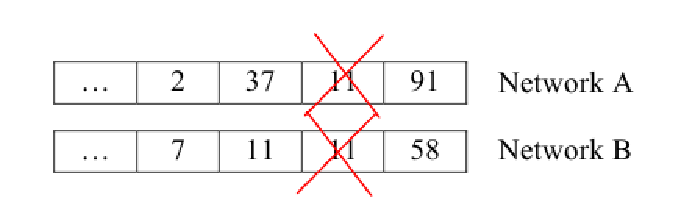
\includegraphics[width=9cm]{mm7_exercise1-1a_cdma.eps}
  \caption{Illustration of collision between two synchronous FH networks. The number denotes the frequency selected in that slot}
  \label{fig:mm7_exercise1-1a_cdma}
\end{figure}

\subsection{a)}
\textit{Find the probability that network A experiences a collision if there are two collocated networks A and B which are synchronous, as on \figref{fig:mm7_exercise1-1a_cdma}}
If the system is synchronous then there will be a collision if the two networks picks the same frequency. For M frequencies the probability will be the probability that B picks every other frequency. 
\begin{flalign}
 && P(coll) =& 1 - P(no coll)& \\
 && \left(1-\frac{M-1}{M}\right) =& \frac{1}{M}&
\end{flalign}


\subsection{b)}
\textit{Find the probability that network A experiences a collision if there are two collocated networks which are asynchronous, as on \figref{fig:mm7_exercise1-1b_cdma}}
\begin{figure}[!h]
  \centering
  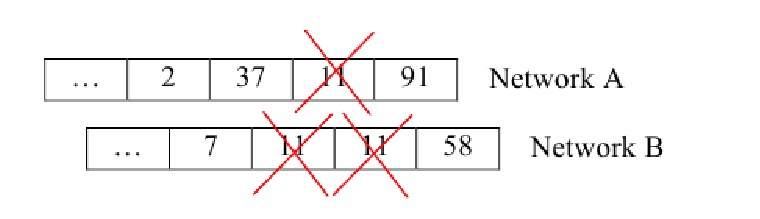
\includegraphics[width=9cm]{mm7_exercise1-1b_cdma.eps}
  \caption{Asynchronous FH networks.}
  \label{fig:mm7_exercise1-1b_cdma}
\end{figure}
\begin{flalign}
 \frac{1}{M}+\frac{1}{M}-\frac{1}{M^{2}} = P_{A} + P_{B} - P(B|A)
\end{flalign}

\subsection{c)}
\textit{Let there be K$>$1 collocated networks, all of them asynchronous with each other. Find the probability that network A experiences a collision.}


\subsection{d)}
\textit{If the number of frequencies is M=80, the number of collocated networks is K=10, each packet carries 100 bytes and the duration of a slot (packet) is TP =50 $\mu$s, find the throughput in [bps] achieved in each network.}
